\documentclass[document.tex]{subfiles} 

\begin{document}

\chapter{برمجة محمل النظام - المرحلة الثانية}
بسبب القيود على حجم محمل النظام فان هذا قد أدى الى تقسيم المهمة الى مرحلتين حيث اقتصرت مهمة المرحلة الاولى على تحميل المرحلة الثانية من المحمل ، أما المرحلة الثانية \en{stage 2} فلا قيود عليها وغالبا ما يتم تنفيذ المهمات التالية في هذه المرحلة:
\begin{itemize}
\item الانتقال الى النمط المحمي\en{PMode}.
\item تفعيل البوابة \en{A20} لدعم ذاكرة حتى \cmd{4} جيجا بايت.
\item توفير دوال للتعامل مع المقاطعات \en{Interrupt Handler}.
\item  تحميل النواة ونقل التنفيذ والتحكم اليها.
\item توفير خصائص أثناء الإقلاع مثل \en{Safe Mode}.
\item دعم الإقلاع المتعدد \en{Multi Boot} وذلك عبر ملفات التهيئة.

\end{itemize}

\section{الانتقال الى النمط المحمي}
المشكلة الرئيسية في النمط الحقيقي \en{Real Mode} هي عدم توفر حماية للذاكرة حيث يمكن لأي برنامج يعمل أن يصل لأي جزء من الذاكرة ، كذلك أقصى حجم يمكن الوصول له هو \cmd{1} ميجا من الذاكرة ، ولا يوجد دعم لتقنية \en{Paging} ولا للذاكرة الظاهرية \en{Virtual Memory} حتى تعدد البرامج لا يوجد دعم له.

كل هذه المشاكل تم حلها باضافة النمط المحمي الى المعالج ويمكن الانتقال بسهولة الى هذا النمط عن طريق تفعيل البت الاول في المسجل \cmd{cr0} ، ولكن بسبب أن المعالج في هذا النمط يستخدم طريقة عنونة للذاكرة تختلف عن الطريقة المستخدمة في النمط الحقيقي فانه يجب تجهيز بعض الجداول تسمى جداول الواصفات \en{Descriptor Table} وبدون تجهيز هذه الجداول فان المعالج سيصدر استثناء \en{General Protection Fault} واختصاراً \en{GPF} والذي بدوره يؤدي الى حدوث \en{triple fault} وتوقف النظام عن العمل.

أحد هذه الجداول ويسمى جدول الواصفات العام  (\en{Global Descriptor Table}) واختصاراً \en{GDT} وظيفته الاساسية هي تعريف كيفية استخدام الذاكرة ، حيث يحدد ما هو القسم الذي سينفذ كشفرة ؟ وما هو القسم الذي يجب أن يحوي بيانات ؟ ويحدد أيضا بداية ونهاية كل قسم بالاضافة الى صلاحية الوصول الى ذلك القسم.

\subsection{جدول الواصفات العام \en{Global Descriptor Table}}
\label{sec:gdt}
عند الانتقال الى النمط المحمي \en{PMode} فان أي عملية وصول الى الذاكرة تتم عن طريق هذا الجدول \en{GDT} ، هذا الجدول يعمل على حماية الذاكرة وذلك بفحص العنوان المراد الوصول اليه والتأكد من عدم مخالفته لبيانات هذا الجدول.هذه البيانات تحدد القسم الذي يمكن أن ينفذ كشفرة (\en{Code}) والقسم الذي لا ينفذ (\en{Data}) كذلك تحدد هذه البيانات العديد من الخصائص كما سنراها الان.

وعادة يتكون جدول \en{GDT} من ثلاث واصفات \en{Descriptors} (حجم كلٌ منها هو \cmd{64} بت) وهم:
\begin{itemize}
\item \en{Null Descriptor}: تكون فارغة في العادة.
\item \en{Code Descriptor}: تصف خصائص المقطع  أو القسم من الذاكرة الذي ينفذ كشفرة \en{Code}.
\item \en{Data Descriptor}: تصف خصائص المقطع أو القسم من الذاكرة الذي لا ينفذ ويحوي بيانات \en{Data}.
\end{itemize}
بيانات أي واصفة \en{Descriptor} تأخذ الجدول التالي:

\begin{itemize}
\item البتات \cmd{0}-\cmd{15}: تحوي أول بايتين (من بت \cmd{0} -\cmd{15}) من حجم المقطع.
\item البتات \cmd{16}-\cmd{39}: تحوي أول ثلاث بايتات من عنوان بداية المقطع \en{Base Address}.
\item البت \cmd{40}: بت الوصول \en{Access Bit} (يستخدم مع الذاكرة الظاهرية \en{Virtual Memory}.
\item البتات \cmd{41-43}: نوع الواصفة \en{Descriptor Type}:
\begin{itemize}
\item البت \cmd{41}: القراءة والكتابة:
\begin{itemize}
\item \en{Data Descriptor}: القيمة \cmd{0} للقراءة فقط والقيمة \cmd{1} للقراءة  والكتابة.
\item \en{Code Descriptor}: القيمة \cmd{0} للتنفيذ فقط \en{execute} والقيمة \cmd{1} للقراءة  والتنفيذ.
\end{itemize}

\item البت \cmd{42}: \en{Expansion direction (Data segments), conforming (Code Segments)}.

\item البت \cmd{43}: قابلية التنفيذ:
\begin{itemize}
\item \cmd{0}: اذا كان المقطع عبارة عن بيانات.
\item \cmd{1}: اذا كان المقطع عبارة عن شفرة.

\end{itemize}
\end{itemize}

\item البت \cmd{44}: \en{Descriptor Bit}:
\begin{itemize}
\item \cmd{0}:\en{System descriptor}.
\item \cmd{1}: \en{Code or Data Descriptor}.

\end{itemize}

\item البتات \cmd{45}-\cmd{46}: مستوى الحماية \en{Privilege Level}
\begin{itemize}
\item \cmd{0}: \en{(Ring 0) Highest}.
\item \cmd{3}: \en{(Ring 3) Lowest}.

\end{itemize}

\item البت \cmd{47}: \en{Segment is in memory (Used with Virtual Memory)}.
\item البتات \cmd{48}-\cmd{51}: تحوي البت \cmd{16} -\cmd{19} من حجم المقطع.
\item البت \cmd{52}: محجوزة.
\item البت \cmd{53}: محجوزة.

\item البت \cmd{54}: نوع المقطع \en{Segment type}:
\begin{itemize}
\item \cmd{0}: اذا كان المقطع \cmd{16} بت.
\item \cmd{1}: اذا كان المقطع \cmd{32} بت.

\end{itemize}

\item البت \cmd{55}: \en{Granularity}:
\begin{itemize}
\item \cmd{0}: \en{None}.
\item \cmd{1}: \en{Limit gets multiplied by 4K}.

\end{itemize}

\item البتات \cmd{56}-\cmd{63}: تحوي البت \cmd{23} -\cmd{32} من عنوان بداية المقطع \en{Base Address}.

\end{itemize}

وفي هذه المرحلة سنقوم ببناء هذا الجدول ويتكون من واصفة للكود وللبيانات \en{Code and Data Descriptor}، بحيث يمكن القراءة و الكتابة من أول بايت في الذاكرة الى آخر الذاكرة \cmd{0xffffffff}. 

\begin{english}
\fontspec{Courier New}
\lstset{numberstyle=\tiny,numbersep=5pt,tabsize=2,extendedchars=true,breaklines=true,frame=b,showspaces=false, showtabs=false,xleftmargin=10pt,framexleftmargin=10pt,framexrightmargin=5pt,framexbottommargin=4pt,showstringspaces=false,language=[x86masm]Assembler}

\lstinputlisting[label=lst:bootloader,caption=Some Code]{../examples/ch3/ex15/ex15.asm}
\end{english}

هذا الجدول يبدأ بالواصفة الخالية \en{Null Descriptor} وحجمها \cmd{8} بايت ومتحوياتها تكون صفراً في العادة ، أما الواصفة التالية لها فهي واصفة مقطع الشفرة \en{Code Descriptor} وتوضح المقطع من الذاكرة الذي سيتسخدم كشفرة وما هي بدايته وحجمه وصلاحيات استخدامه حيث يمكن أن نسمح فقط للبرامج التي تعمل على مستوى النواة \en{Kernel Mode} بالدخول الى هذا المقطع.وفيما يلي شرح لمحتويات هذه الواصفة ويمكنك المطابقة مع الجدول الذي يوضح الشكل العام لكل واصفة.

تبدأ واصفة الكود \en{Code Descriptor} من العنوان \cmd{0x8} وهذا العنوان مهم جدا حيث سيكون هذا العنوان هو قيمة المسجل \cmd{CS} ، والبتات من \cmd{0}-\cmd{15} تحدد حجم المقطع \en{Segment Limit} والقيمة هي \cmd{0xffff} تدل على أن أكبر حجم يمكن التعامل معه هو \cmd{0xffff}.

البتات من \cmd{16}-\cmd{39} تمثل البتات \cmd{0}-\cmd{23} من عنوان بداية المقطع \en{Base Address} والقيمة التي تم اختيارها هي \cmd{0x0} وبالتالي نعرف أن عنوان بداية مقطع الكود هو \cmd{0x0} وعنوان النهاية \en{0xffff} .

البايت رقم \cmd{6} ويسمى \en{Access Byte} يحدد العديد من الخصائص وفيما يلي توضيح لمعنى كل بت موجودة فيه:
\begin{itemize}
\item البت \cmd{0}: \en{Access Bit} ويستخدم مع الذاكرة الظاهرية لذلك اخترنا القيمة \cmd{0}.
\item البت \cmd{1}: بت القراءة والكتابة ، وتم اختيار القيمة \cmd{1} لذا يمكن قراءة وتنفيذ أي بايت موجودة في مقطع الكود من \cmd{0x0}-\cmd{0xffff}.
\item البت \cmd{2}: \en{expansion direction} لا يهم حاليا لذا القيمة هي \cmd{0}.
\item البت \cmd{3}: تم اختيار القيمة \cmd{1} دلالة على أن هذا مقطع شفرة \en{Code Segment}.
\item البت \cmd{4}: تم اختيار القيمة \cmd{1} دلالة على أن هذا مقطع للشفرة او للبيانات وليس للنظام.
\item البتات \cmd{5}-\cmd{6}: مستوى الحماية وتم اختيار القيمة \cmd{0} دلالة على أن هذا المقطع يستخدم فقط في الحلقة صفر \en{Ring0} أو ما يسمى \en{Kernel Mode}.
\item البت \cmd{7}: تستخدم مع الذاكرة الظاهرية لذا تم اهمالها.
\end{itemize}

البايت رقم \cmd{7} ويسمى \en{granularity } يحدد أيضا بعض الخصائص، وفيما يلي توضيح لمعنى كل بت موجودة فيه:

\begin{itemize}
\item البتات \cmd{0}-\cmd{3}: تمثل البتات من \cmd{16}-\cmd{19} من نهاية حجم المقطع \en{Segment Limit} والقيمة هي \cmd{0xf} ، وبهذا يكون أقصى عنوان للمقطع هو \cmd{0xfffff} أي \cmd{1} ميجا من الذاكرة ، ولاحقاً عندما يتم تفعيل بوابة \en{A20} سنتمكن من الوصول حتى \cmd{4} جيجا من الذاكرة.

\item البتات \cmd{4}-\cmd{5}: محجوزة للنظام لذا تم اهمالها.
\item البت \cmd{6}: تم اختيار القيمة \cmd{1} دلالة على هذا المقطع هو \cmd{32} بت.
\item البت \cmd{7}: باختيار القيمة \cmd{1} سيتم إحاطة المقطع ب \cmd{4 KB}.

\end{itemize}

البايت الاخير في واصفة مقطع الكود (البايت رقم \cmd{8}) يمثل البتات من \cmd{24}-\cmd{32} من عنوان بداية مقطع الكود والقيمة هي \cmd{0x0} وبالتالي عنوان بداية مقطع الكود الكلي هو \cmd{0x0} أي من أول بايت في الذاكرة.

إذاً واصفة مقطع الكود  \en{Code Descriptor} حددت عنوان بداية مقطع الكود ونهايته وكذلك صلاحية التنفيذ وحددت بأن المقطع هو مقطع كود \en{Code Segment}.

الواصفة التالية هي واصفة مقطع البيانات  \en{Data Descriptor} وتبدأ من العنوان رقم \cmd{0x10} وهي مشابهة تماما لواصفة الكود باستثناء البت رقم \cmd{43} حيث يحدد ما اذا كان المقطع كود أم بيانات.

وبعد إنشاء هذا الجدول (\en{GDT}) في الذاكرة ، يجب أن يَحمِل المسجل \cmd{gdtr}  على حجم هذا الجدول ناقصا واحد وعلى عنوان بداية الجدول، ويتم ذلك عن طريق إنشاء مؤشرا الى جدول \en{GDT} ومن ثم  استخدام الامر \cmd{lgdt} (وهو أمر يعمل فقط في الحلقة صفر \en{Ring0}) ، والشفرة التالية توضح ذلك.

\begin{english}
\fontspec{Courier New}
\lstset{numberstyle=\tiny,numbersep=5pt,tabsize=2,extendedchars=true,breaklines=true,frame=b,showspaces=false, showtabs=false,xleftmargin=10pt,framexleftmargin=10pt,framexrightmargin=5pt,framexbottommargin=4pt,showstringspaces=false,language=[x86masm]Assembler}

\lstinputlisting[label=lst:bootloader,caption=Some Code]{../examples/ch3/ex16/ex16.asm}
\end{english}

\subsection{العنونة في النمط المحمي \en{PMode Memory Addressing}}
في النمط الحقيقي يستخدم المعالج عنونة \en{Segment:Offset} وذلك بأن تكون أي من مسجلات المقاطع (\en{Segments Registers}) تحوي عنوان بداية المقطع ، ومسجلات العناوين تحوي العنوان داخل مقطع ما ، ويتم ضرب عنوان المقطع بالعدد \en{0x10} وجمع ال \en{offset} اليه للحصول على العنوان النهائي والذي سيمر بداخل مسار العنوان \en{Address Bus}.

أما النمط المحمي \en{PMode} فانه يستخدم عنونة \en{Descriptor:Offset} وذلك بأن تكون مسجلات المقاطع تحوي عنوان أحد الواصفات التي قمنا ببنائها (مثلا مسجل \cmd{CS} يحوي العنوان \cmd{0x8} ومسجل البيانات \cmd{DS} يحوي العنوان \cmd{0x10}) ، وال \en{offset} سيتم جمعها الى عنوان بداية المقطع  \en{Base Address} والذي قمنا بتحديده في جدول الواصفات كذلك سيتم التأكد من أن هذا العنوان لا يتجاوز حجم المقطع \en{Segment Limit} أيضا سيتم التأكد من مستوى الصلاحية وأنه يمكن الوصول للعنوان المطلوب. ونظراً لان في النمط المحمي يمكن استخدام مسجلات \cmd{32-bit} فانه يمكن عنونة \cmd{4} جيجا من الذاكرة\footnote{بفرض أن بوابة \en{A20} تم تفعيلها.}.

 
\subsection{الانتقال الى النمط المحمي}
بعد إنشاء جدول \en{GDT} وتحميل مسجل \en{GDTR} يمكن الانتقال الى النمط المحمي عن طريق تفعيل البت الاول في مسجل التحكم \cmd{cr0}، وكما هو معروف أن هذا النمط لا يستخدم مقاطعات البايوس لذا يجب تعطيل عمل المقاطعات قبل الانتقال حتى لا تحدث أي مشاكل.

وبعد الانتقال الى النمط المحمي فان يجب تعيين الواصفة التي يجب استخدامها لمسجلات المقاطع ، وبالنسبة لمسجل \cmd{CS} فانه يمكن تعديل قيمته وذلك عن طريق تنفيذ \en{far jump} ،والكود التالي يوضح طريقة الانتقال الى النمط المحمي وتعديل قيم مسجلات المقاطع.

 
\begin{english}
\fontspec{Courier New}
\lstset{numberstyle=\tiny,numbersep=5pt,tabsize=2,extendedchars=true,breaklines=true,frame=b,showspaces=false, showtabs=false,xleftmargin=10pt,framexleftmargin=10pt,framexrightmargin=5pt,framexbottommargin=4pt,showstringspaces=false,language=[x86masm]Assembler}

\lstinputlisting[label=lst:bootloader,caption=Some Code]{../examples/ch3/ex17/ex17.asm}
\end{english}


\section{تفعيل البوابة \en{A20}}
بوابة \en{A20 Gate} هي عبارة عن \en{OR Gate} موجودة على ناقل النظام \en{System Bus} \footnote{توجد البوابة تحديداً على خط العناوين رقم \cmd{20}}والهدف منها هو التحكم في عدد خطوط العناوين \en{Address Line}، حيث كانت الاجهزة قديما (ذات المعالجات التي تسبق معالج \cmd{80286}) تحوي على \cmd{20} بت (خط) للعناوين (\en{20 address line}) ، وعندما صدرت اجهزة \en{IBM PC} والتي احتوت على معالج \en{80286} تم زيادة خط العناوين الى \cmd{32} خط وهكذا أصبح من الممكن عنونة \cmd{4} جيجا من الذاكرة ، وحتى يتم الحفاظ على التوافقية مع الاجهزة السابقة فانه يمكن التحكم في بوابة \en{A20} من فتح الخطوط \en{A20}-\en{A31} واغلاقها.

هذه البوابة مرتبطة مع متحكم \cmd{8042} وهو متحكم لوحة المفاتيح (\en{Keyboard Controller}) ، وعند تفعيل البت رقم \cmd{1} في منفذ خروج البيانات (\en{output data port}) التابع لمتحكم لوحة المفاتيح فان هذا يفتح بوابة \en{A20} وبهذا نستطيع الوصول الى \cmd{4} جيجا من الذاكرة ، ابتداءاً من العنوان \cmd{0x0}-\cmd{0xffffffff} 

وعند اقلاع الحاسب فان البايوس يقوم بتفعيل هذه البوابة لأغراض حساب حجم الذاكرة واختبارها ومن ثم يقوم بغلقها مجدداً للحفاظ على التوافقية مع الاجهزة القديمة.

وتوجد العديد من الطرق لتفعيل هذه البوابة ، العديد منها يعمل على أجهزة معينة لذلك سيتم ذكر العديد من الطرق واستخدام أكثر الطرق محمولية على صعيد الاجهزة المختلفة.

\subsection{متحكم لوحة المفاتيح \en{8042} والبوابة \en{A20}}
عند الانتقال الى النمط المحمي (\en{PMode}) فانه لن يمكن استخدام مقاطعات البايوس ويجب التعامل المباشر مع متحكم أي عتاد والقراءة والكتابة من مسجلات المتحكم الداخلية . وبسبب ارتباط بوابة \en{A20} مع متحكم لوحة المفاتيح فانه لا بد من التعامل مع هذا المتحكم لتفعيل البوابة ، وهذا يتم عن طريق استخدام أوامر المعالج \en{in} والامر \en{out}.

وبخصوص متحكم لوحة المفاتيح (متحكم \en{8042}) فغالبا ما تأتي على شكل شريحة \en{Integrated Circuit} أو تكون مضمنة داخل اللوحة الأم (\en{Motherboard}) وتكون في ال \en{South Bridge}.ويرتبط هذا المتحكم مع متحكم آخر بداخل لوحة المفاتيح ، وعند الضغط على زر ما فانه يتم توليد \en{Make Code} ويُرسل الى المتحكم الموجود بداخل لوحة المفاتيح والذي بدروه يقوم بارساله الى متحكم \en{8042} عن طريق منفذ الحاسب (\en{Hardware Port}) .وهنا يأتي دور متحكم \en{8042} حيث يقوم بتحويل \en{Make code} الى \en{Scan Code} ويحفظها في مسجلاته الداخلية \en{Buffer} هذا المسجل يحمل الرقم \cmd{0x60} في أجهزة \en{IBM and Compatible PC}، وهذا يعني أنه في حالة قراءة هذا المسجل (عن طريق الأمر \cmd{in}) فانه يمكن قراءة القيمة المدخلة.

وفي الفصل السادس سيتم مناقشة متحكم لوحة المفاتيح بالتفصيل ، وسنكتفي هنا فقط بتوضيح الأجزاء المتعلقة بتفعيل بوابة \en{A20}.



\subsection{طرق تفعيل البوابة \en{A20}}

\subsubsection{بواسطة \en{System Control Port 0x92}}

في بعض الاجهزة يمكن استخدام أحد منافذ الادخال والاخراج وهو \en{I/O part 0x92} لتفعيل بوابة \en{A20} ، وعلى الرغم من سهولة هذه الطريقة الا أنها تعتبر أقل محمولية وبعض الاجهزة لا تدعمها ، وفيما يلي توضيح للبتات على هذا المنفذ:

\begin{itemize}
\item البت \cmd{0}: تفعيل هذا البت يؤدي الى عمل \en{reset} للنظام والعودة الى النمط الحقيقي.
\item البت \cmd{1}: القيمة \cmd{0} لتعطيل بوابة \en{A20} ، والقيمة \cmd{1} لتفعيلها.
\item البت \cmd{2}: لا تستخدم.
\item البت \cmd{3}: \en{power on password bytes}
\item البتات \cmd{4}-\cmd{5}: لا تستخدم.
\item البتات \cmd{6}-\cmd{7}: \en{HDD activity LED} : القيمة \cmd{0}: \en{off}، القيمة \cmd{1}: \en{on}.
\end{itemize} 

والمثال التالي يوضح طريقة تفعيل البوابة .


\begin{english}
\fontspec{Courier New}
\lstset{numberstyle=\tiny,numbersep=5pt,tabsize=2,extendedchars=true,breaklines=true,frame=b,showspaces=false, showtabs=false,xleftmargin=10pt,framexleftmargin=10pt,framexrightmargin=5pt,framexbottommargin=4pt,showstringspaces=false,language=[x86masm]Assembler}

\lstinputlisting[label=lst:bootloader,caption=Some Code]{../examples/ch3/ex18/ex18.asm}
\end{english}

ويجب ملاحظة أن هذه الطريقة لا تعمل في كل الاجهزة وربما يكون هناك ارقام مختلفة للمنافذ ، ويعتمد في الآخر على مصنعي اللوحات الام ويجب قراءة كتيباتها لمعرفة العناوين.

\subsubsection{بواسطة البايوس}
يمكن استخدام مقاطعة البايوس \cmd{int 0x15} الدالة \cmd{0x2401} لتفعيل بوابة \en{A20} ، والدالة \cmd{0x2400} لتعطيلها.مع التذكير بأن يجب أن يكون المعالج في النمط الحقيقي حتى نتمكن من استدعاء هذه المقاطعة، والكود التالي يوضح طريقة التفعيل باستخدام البايوس.

\begin{english}
\fontspec{Courier New}
\lstset{numberstyle=\tiny,numbersep=5pt,tabsize=2,extendedchars=true,breaklines=true,frame=b,showspaces=false, showtabs=false,xleftmargin=10pt,framexleftmargin=10pt,framexrightmargin=5pt,framexbottommargin=4pt,showstringspaces=false,language=[x86masm]Assembler}

\lstinputlisting[label=lst:bootloader,caption=Some Code]{../examples/ch3/ex19/ex19.asm}
\end{english}

\subsubsection{بواسطة متحكم لوحة المفاتيح}
يوجد منفذين لمتحكم لوحة المفاتيح: المنفذ \cmd{0x60} وهو يمثل ال \en{buffer} (في حالة القراءة منه يسمى \en{Output Buffer} وفي حالة الكتابة يسمى \en{Input Buffer}، والمنفذ \cmd{0x64} وهو لإرسال الاوامر الى المتحكم ولقراءة حالة المتحكم (\en{Status}). حيث يتم ارسال الأوامر الى المتحكم عن طريق المنفذ \cmd{0x64} واذا كان هناك وسائط لهذا الأمر فترسل الى ال \en{buffer} (المنفذ \cmd{0x60}) وكذلك تقرأ النتائج من المنفذ \cmd{0x60}.

وحيث ان تنفيذ أوامر البرنامج (عن طريق المعالج) أسرع بكثير من تنفيذ الأوامر المرسلة الى متحكم لوحة المفاتيح (وبشكل عام الى أي متحكم لعتاد ما)  فانه يجب ان نوفر طرقاً لانتظار المتحكم قبل العودة الى البرنامج لاستكمال التنفيذ .

ويمكن عن طريق قراءة حالة المتحكم (عن طريق قراءة المنفذ \cmd{0x64}) أن نعرف ما اذا تم تنفيذ الاوامر المرسلة ام لا ، وكذلك هل هناك نتيجة لكي يتم قرائتها في البرنامج ام لا.

وما يهمنا من البتات عند قراءة حالة المتحكم حاليا هو أول بتين فقط  ، ووظيفتهما هي:

\begin{itemize}
\item البت \cmd{0}: حالة ال \en{Output Buffer}:
\begin{itemize}
\item القيمة \cmd{0}: ال \en{Output Buffer} خالي (لا توجد نتيجة ، لا تقرأ الان).
\item القيمة \cmd{1}: ال \en{Output Buffer} ممتلئ (توجد نتيجة ، قم بالقراءة الان).
\end{itemize}

\item البت \cmd{1}: حالة ال \en{Input Buffer}:
\begin{itemize}
\item القيمة \cmd{0}: ال \en{Input Buffer} خالي (لا توجد أوامر غير منفذة ، يمكن الكتابة الان).
\item القيمة \cmd{1}: ال \en{Input Buffer} ممتلئ (توجد أوامر غير منفذة ، لا تكتب الان).
\end{itemize}

\end{itemize}

والشفرة التالية توضح كيفية انتظار المتحكم حتى ينفذ الاوامر المرسله اليه (\en{wait input}) وكيفية انتظار المتحكم الى ان يأتي بنتيجة ما (\en{wait output}).

\begin{english}
\fontspec{Courier New}
\lstset{numberstyle=\tiny,numbersep=5pt,tabsize=2,extendedchars=true,breaklines=true,frame=b,showspaces=false, showtabs=false,xleftmargin=10pt,framexleftmargin=10pt,framexrightmargin=5pt,framexbottommargin=4pt,showstringspaces=false,language=[x86masm]Assembler}

\lstinputlisting[label=lst:bootloader,caption=Some Code]{../examples/ch3/ex20/ex20.asm}
\end{english}

ولإرسال اوامر الي المتحكم فان يجب استخدام المنفذ \cmd{0x64} وتوجد الكثير من الأوامر ، ونظرا لان هذا الجزء غير مخصص لبرمجة متحكم لوحة المفاتيح فاننا سنناقش فقط الاوامر التي تهمنا حاليا ، وفي الفصل السادس سنعود الى الموضوع بالتفصيل ان شاء الله.

وقائمة الاوامر حاليا:
\begin{itemize}
\item الأمر \cmd{0xad}: تعطيل لوحة المفاتيح.
\item الأمر \cmd{0xae}: تفعيل لوحة المفاتيح.
\item الأمر \cmd{0xd0}: القراءة من \en{Output Port}.
\item الأمر \cmd{0xd1}: الكتابة الى \en{Output Port}.
\item الأمر \cmd{0xdd}: تفعيل بوابة \en{A20}.
\item الأمر \cmd{0xdf}: تعطيل بوابة \en{A20}.

\end{itemize}

وعن طريق الأمر \cmd{0xdd} فانه يمكن تفعيل البوابة \en{A20} بسهولة كما في الشفرة التالية ، لكن أيضا هذه الطريقة لا تعمل على كل الاجهزة حيث هناك بعض المتحكمات لا تدعم هذا الأمر.

\begin{english}
\fontspec{Courier New}
\lstset{numberstyle=\tiny,numbersep=5pt,tabsize=2,extendedchars=true,breaklines=true,frame=b,showspaces=false, showtabs=false,xleftmargin=10pt,framexleftmargin=10pt,framexrightmargin=5pt,framexbottommargin=4pt,showstringspaces=false,language=[x86masm]Assembler}

\lstinputlisting[label=lst:bootloader,caption=Some Code]{../examples/ch3/ex21/ex21.asm}
\end{english}

وتوجد طريقة أخرى أكثر محمولية وهي عن طريق منفذ الخروج \en{Output Port} في متحكم لوحة المفاتيح ويمكن قراءة هذا المنفذ والكتابة اليه عن طريق ارسال الاوامر \cmd{0xd0} و \cmd{0xd1} على التوالي.

وعند قراءة هذا المنفذ (بارسال الامر \cmd{d0} الى متحكم لوحة المفاتيح) فان القيم تعني:

\begin{itemize}
\item البت \cmd{0}: \en{System Reset}:
\begin{itemize}
\item القيمة \cmd{0}: \en{Reset Computer}.
\item القيمة \cmd{1}: \en{Normal Operation}.
\end{itemize}

\item البت \cmd{1}: بوابة \en{A20}:
\begin{itemize}
\item القيمة \cmd{0}: تعطيل.
\item القيمة \cmd{1}: تفعيل.
\end{itemize}

\item البتات \cmd{2}-\cmd{3}: غير معرف.
\item البت \cmd{4}: \en{Input Buffer Full}.
\item البت \cmd{5}: \en{Output Buffer Empty}.
\item البت \cmd{6}: \en{Keyboard Clock}:
\begin{itemize}
\item القيمة \cmd{0}: \en{High-Z}.
\item القيمة \cmd{1}: \en{Pull Clock Low}.
\end{itemize}

\item البت \cmd{7}: \en{Keyboard Data}:
\begin{itemize}
\item القيمة \cmd{0}: \en{High-Z}.
\item القيمة \cmd{1}: \en{Pull Data Low}.
\end{itemize}
\end{itemize}

وعند تفعيل البت رقم \cmd{1} فان هذا يفعل بوابة \en{A20} ويجب استخدام الامر \cmd{or} حتى يتم الحفاظ على بقية البتات .وبعد ذلك يجب كتابة القيم الى نفس المنفذ باستخدام الامر \cmd{0xd1} .

والشفرة التالية توضح كيفية تفعيل بوابة \en{A20} عن طريق منفذ الخروج \en{Output Port} لمتحكم لوحة المفاتيح.

\begin{english}
\fontspec{Courier New}
\lstset{numberstyle=\tiny,numbersep=5pt,tabsize=2,extendedchars=true,breaklines=true,frame=b,showspaces=false, showtabs=false,xleftmargin=10pt,framexleftmargin=10pt,framexrightmargin=5pt,framexbottommargin=4pt,showstringspaces=false,language=[x86masm]Assembler}

\lstinputlisting[label=lst:bootloader,caption=Some Code]{../examples/ch3/ex22/ex22.asm}
\end{english}

حيث في البداية تم تعطيل لوحة المفاتيح (عن طريق ارسال الامر \cmd{0xad}) واستدعاء الدالة \en{wait input} للتأكد من أن الامر قد تم تنفيذه ومن ثم تم ارسال أمر قراءة منفذ الخروج لمتحم لوحة المفاتيح (الامر \cmd{0xda}) وانتظار المتحكم حتى ينتهي من تنفيذ الامر ، وقد تم استخدام الدالة \en{wait output} لانتظار قيمة منفذ الخروج ، وبعدها تم قراءة هذه القيمة وحفظها في المكدس (\en{Stack}) ،وبعد ذلك تم ارسال أمر الكتابة الى منفذ الخروج لمتحكم لوحة المفاتيح (الامر \cmd{0xd1}) وانتظار المتحكم حى ينتهي من تنفيذ الامر ومن قمنا بارسال قيمة المنفذ الخروج الجديدة بعد أن تم تفعيل البت رقم \cmd{1} وهو البت الذي يفعل بوابة \en{A20} ، وفي الاخير تم تفعيل لوحة المفاتيح مجددا.
 

\section{أساسيات ال \en{VGA}}
في عام \en{1987} قامت \en{IBM} بتطوير مقياس لمتحكمات شاشة الحاسب وهو \en{Video Graphics Array} واختصاراً \en{VGA} وجائت تسميته ب \en{Array} نظرا لانه تم تطويره كشريحة واحدة \en{signle chip} حيث استبدلت العديد من الشرائح والتي كانت تستخدم في مقاييس اخرى مثل \en{MDA} و \en{CGA} و \en{EGA} ، ويتكون ال \en{VGA} من \en{Video Buffer}, \en{Video DAC} , \en{CRT Controller} , \en{Sequencer unit} , \en{Graphics Controller} و \en{Attribute Controller}\footnote{شرح هذه المكونات سيكون في الفصل الخامس باذن الله ، وسيتم التركيز على بعض الاشياء بحسب الحاجة حاليا.}.

ال \en{Video Buffer} هو مقطع من الذاكرة \en{segment of memory} يعمل كذاكرة للشاشة \en{Memory Mapped} ، وعند بداية التشغيل فان البايوس يخصص مساحة من الذاكرة بدءا من العنوان \cmd{0xa0000} كذاكرة للشاشة وفي حالة تم الكتابة الى هذه الذاكرة فان هذا سوف يغير في الشاشة ، هذا الربط يسمى \en{Memory Mapping}، أما ال \en{Graphics Controller} فهو الذي يقوم بتحديث محتويات الشاشة بناءاً على البيانات الموجودة في ال \en{Video buffer}.
 
وتدعم ال \en{VGA} نمطين للعرض الاول هو النمط النصي \en{Text Mode} والاخر هو النمط الرسومي \en{APA Graphics Mode} ويحدد النمط طريقة التعامل مع ال \en{Video buffer} وكيفة عرض البيانات.

النمط الرسومي \en{All Point Addressable Graphics Mode} يعتمد على البكسلات ، حيث يمكن التعامل مع كل بسكل موجود على حدة . والبكسل هو أصغر وحدة في الشاشة وتعادل نقطة على الشاشة. أما النمط النصي \en{Text Mode} فيعتمد على الحروف \en{Characters} ، ولتطبيق هذا النمط فان متحكم الشاشة \en{Video Controller} يستخدم ذاكرتين \en{two buffers} الاولى وهي خريطة الحروف \en{Character Map} وهي تعرف البكسلات لكل حرف ويمكن تغيير هذه الخريطة لدعم أنظمة محارف أخرى، أما الذاكرة الثانية فهي\en{Screen Buffer} وبمجرد الكتابة عليها فان التأثير سيظهر مباشرة على الشاشة.

ومقياس \en{VGA} هو مبني على المقاييس السابقة ، ابتداءا من مقياس \en{Monochrome Display Adapter} ويسمى اختصارا \en{MDA} والذي طورته \en{IBM} في عام \en{1981} ، و \en{MDA} لا تدعم النمط الرسومي والنمط النصي بها (يسمى \en{Mode 7}) يدعم \en{80} عمود و \en{24} صف ( \cmd{25*80}). وفي نفس العام قامت \en{IBM} بتطوير مقياس \en{Color Graphics Adapter} (واختصارا \en{CGA}) الذي كان أول متحكم يدعم الالوان حيث يمكن عرض \en{16} لون مختلف.وبعد ذلك تم تطوير \en{Enhanced Graphics Adapter}.

ويجدر بنا التذكير بان متحكمات \en{VGA} متوافقة مع المقاييس السابقة \en{Backward Compatible} فعندما يبدأ الحاسب في العمل فان النمط سيكون النمط النصي \en{Mode 7} (الذي ظهر في \en{MDA}) ، وهذا يعني اننا سنتعامل مع \en{80} عمود و \en{25} صف.


\subsection{عنونة الذاكرة في متحكمات \en{VGA}}

عندما يبدأ الحاسب بالعمل فان البايوس يخصص العناوين من \cmd{0xa0000} الى \cmd{0xbffff} لذاكرة الفيديو \en{Video memroy} (موجودة على متحكم \en{VGA}) ، هذه العناوين مقسمة كالاتي:

\begin{itemize}
\item من \cmd{0xb0000} الى \cmd{0xb7777}: للنمط النصي أحادي اللون \en{Monochrome Text Mode}.
\item من \cmd{0xb8000} الى \cmd{0xbffff}: \en{Color Text Mode}.
\end{itemize}

وعند الكتابة في هذه العناوين فان هذا سوف يؤثر في الشاشة واظهار القيم التي تم كتابتها ، والمثال التالي يوضح كيفية كتابة حرف \en{A} بلون أبيض وخلفية سوداء.

\begin{english}
\fontspec{Courier New}
\lstset{numberstyle=\tiny,numbersep=5pt,tabsize=2,extendedchars=true,breaklines=true,frame=b,showspaces=false, showtabs=false,xleftmargin=10pt,framexleftmargin=10pt,framexrightmargin=5pt,framexbottommargin=4pt,showstringspaces=false,language=[x86masm]Assembler}

\lstinputlisting[label=lst:bootloader,caption=Some Code]{../examples/ch3/ex23/ex23.asm}
\end{english}

\subsection{طباعة حرف على الشاشة}
لطباعة حرف على الشاشة يجب ارسال الحرف الى عنوان ال \en{Video Memory} وحتى نتمكن من طباعة العديد من الحروف فانه يجب انشاء متغيران (\en{x,y}) لحفظ المكان الحالي للصف والعمود ومن ثم تحويل هذا المكان الى عنوان في ال \en{Video Memoey}. وفي البداية ستكون قيم (\en{x,y}) هي (\cmd{0,0}) أي ان الحرف سيكون في الجزء الاعلي من اليسار في الشاشة ويجب ارسال هذا الحرف الى عنوان بداية ال \en{Video Memory} وهو \cmd{0xb8000} (\en{Color text Mode}). ولطباعة حرف آخر فان قيم (\en{x,y}) له هي (\cmd{0,1})  ويجب ارسال الحرف الى العنوان \cmd{0xb8001} ، وسنستخدم العلاقة التالية للتحويل بين قيم (\en{x,y}) الى عناوين لذاكرة العرض \en{Video Memory}:

\begin{english}
\en{$video memory = 0xb0000$}\\
\en{$video memory += x + y*80$}\\
\end{english}

وبسبب أن هناك \cmd{80} حرف في كل عمود فانه يجب ضرب قيمة \en{y} ب \cmd{80} . والمثال التالي يوضح كيفية طباعة حرف عند (\en{4,4}) .

\begin{english}
\en{$address = x + y*80$}\\

\en{$address = 4 +4*80 = 324$}\\

\en{; now add the base address of video memory.}\\

\en{$address = 324 + 0xb8000 = 0xb8144$}\\
\end{english}

وبارسال الحرف الى العنوان \cmd{ 0xb8144} فان الحرف سوف يظهر على الشاشة في الصف الخامس والعمود الخامس (الترقيم يبدأ من صفر وأول صف وعمود رقمها صفر).
 

وكما ذكرنا ان النمط النصي \en{Mode 7} هو الذي يبدأ الحاسب به ، في هذا النمط يتعامل متحكم العرض مع بايتين من الذاكرة لكل حرف يراد طباعته ، بمعنى اذا ما أردنا طباعة الحرف \en{A} فانه يجب ارسال الحرف الى العنوان \cmd{0xb8000} وخصائص الحرف الى العنوان التالي له \cmd{0xb8001} وهذا يعني انه يجب تعديل قانون التحويل السابق واعتبار أن كل حرف يأخذ بايتين من الذاكرة وليس بايت واحد.

البايت الثاني للحرف يحدد لون الحرف وكثافة اللون (غامق وفاتح) والجدول التالي يوضح البتات فيه:

\begin{itemize}
\item البتات \cmd{0}-\cmd{2}: لون الحرف:
\begin{itemize}
\item البت \cmd{0}: أحمر.
\item البت \cmd{1}: أخضر.
\item البت \cmd{2}: أزرق.

\end{itemize}

\item البت \cmd{3}: كثافة لون الحرف ( \cmd{0} غامق ، \cmd{1} فاتح).
\item البت \cmd{4}-\cmd{6}: لون خلفية الحرف:
\begin{itemize}
\item البت \cmd{0}: أحمر.
\item البت \cmd{1}: أخضر.
\item البت \cmd{2}: أزرق.

\end{itemize}
\item البت \cmd{7}: كثافة لون خلفية الحرف ( \cmd{0} غامق ، \cmd{1} فاتح).


\end{itemize}

وهكذا توجد \cmd{4} بت لتحديد اللون ، والجدول التالي يوضح هذه الألوان:
\begin{english}
\begin{itemize}
\item \en{0: Black}.
\item \en{1: Blue}.
\item \en{2: Green}.
\item \en{3: Cyan}.
\item \en{4: Red}.
\item \en{5: Magneta}.
\item \en{6: Brown}.
\item \en{7: Light gray}.
\item \en{8: Dark Gray}.
\item \en{9: Light Blue}.
\item \en{10: Light Green}.
\item \en{11: Light Cyan}.
\item \en{12: Light Red}.
\item \en{13: Light Magneta}.
\item \en{14: Light Brown}.
\item \en{15: White}.

\end{itemize}
\end{english}

اذاً لطباعة حرف على النمط \en{Mode 7} فانه يجب ارسال الحرف وخصائصه الى ذاكرة العرض ، كما يجب مراعاة بعض الامور من تحديث المؤشر \en{Cursor} (هو خط  \en{underline} يظهر ويختفي للدلالة على الموقع الحالي) و الانتقال الى الصف التالي في حالة الوصول الى اخر حرف في العمود أو في حالة كان الحرف المراد طباعته هو حرف الانتقال الى سطر جديد \en{0xa} . والمثال التالي يوضح الدالة \en{putch32} والتي تستخدم لطباعة حرف على الشاشة في النمط المحمي \en{PMode}.

\begin{english}
\fontspec{Courier New}
\lstset{numberstyle=\tiny,numbersep=5pt,tabsize=2,extendedchars=true,breaklines=true,frame=b,showspaces=false, showtabs=false,xleftmargin=10pt,framexleftmargin=10pt,framexrightmargin=5pt,framexbottommargin=4pt,showstringspaces=false,language=[x86masm]Assembler}

\lstinputlisting[label=lst:bootloader,caption=Some Code]{../examples/ch3/ex24/ex24.asm}
\end{english}

وتبدأ هذه الدالة بفحص الحرف المراد طباعته (موجود في المسجل \cmd{bl}) مع حرف الانتقال الى السطر الجديد \cmd{0xa} وفي حالة التساوي يتم نقل التنفيذ الى آخر جسم الدالة والذي يقوم بتصفير قيمة \en{x} وزيادة قيمة \en{y} دلالة على الانتقال الى السطر الجديد. أما في حالة كان الحرف هو أي حرف آخر فانه يجب حساب العنوان الذي يجب ارسال الحرف اليه حتى يمكن طباعته ، وكما ذكرنا أن النمط النصي \en{Mode 7} يستخدم بايتين لكل حرف لذا سيتم استخدام العلاقة التالية للتحويل ما بين (\en{x,y}) الى العنوان المطلوب.

\begin{english}
\en{$video memory = 0xb0000$}\\
\en{$video memory += x*2 + y*80*2$}\\
\end{english}

وكما يظهر في الكود السابق فقد تم حساب هذا العنوان وحفظه في المسجل \cmd{eax}  وبعد ذلك تم طباعة الحرف المطلوب بالخصائص التي تم تحديدها مسبقا كثابت. وآخر خطوة في الدالة هي زيادة قيم (\en{x,y}) للدالة الى المكان التالي ، وهذا يتم بزيادة \en{x} فقط وفي حالة تساوت القيمة مع قيمة آخر عمود في الصف فانه يتم زيادة قيمة \en{y} وتصفير \en{x} دلالة على الانتقال الى الصف التالي.

\subsection{طباعة السلاسل النصية \en{strings}}
لطباعة سلسلة نصية سنستخدم دالة طباعة الحرف وسنقوم بأخذ حرف حرف من السلسة وارسالها الى دالة طباعة الحرف حتى تنتهي السلسلة ، والشفرة التالية توضح الدالة \en{puts32} لطباعة سلسلة نصية.

\begin{english}
\fontspec{Courier New}
\lstset{numberstyle=\tiny,numbersep=5pt,tabsize=2,extendedchars=true,breaklines=true,frame=b,showspaces=false, showtabs=false,xleftmargin=10pt,framexleftmargin=10pt,framexrightmargin=5pt,framexbottommargin=4pt,showstringspaces=false,language=[x86masm]Assembler}

\lstinputlisting[label=lst:bootloader,caption=Some Code]{../examples/ch3/ex25/ex25.asm}
\end{english}

في هذه الدالة سيتم قراءة حرف حرف من السلسة النصية وطباعته الى أن نصل الى نهاية السلسلة (القيمة \cmd{0x0}) ، وبعد ذلك سيتم تحديث المؤشر وذلك عن طريق متحكم \en{CRT Controller} ونظراً لان التعامل معه بطئ قليلا فان تحديث المؤشر سيكون بعد طباعة السلسلة وليس بعد طباعة كل حرف .

\subsection{تحديث المؤشر \en{Hardware Cursor}}
عند طباعة حرف او سلسلة نصية فان مؤشر الكتابة لا يتحرك من مكانه الا عند تحديده يدويا ، وهذا يتم عن طريق التعامل مع متحكم \en{CRT Controller} . هذا المتحكم يحوي العديد من المسجلات ولكننا سوف نركز على مسجل البيانات \en{Data Register} ومسجل نوع البيانات \en{Index Register}.

ولارسال بيانات الى هذا المتحكم ، فيجب اولا تحديد نوع البيانات وذلك بارسالها الى مسجل \en{Index Register} ومن ثم ارسال البيانات الى مسجل البيانات \en{Data Register} ، وفي حواسيب \en{x86} فان مسجل البيانات يأخذ العنوان \cmd{0x3d5} ومسجل \en{Index Register} يأخذ العنوان \cmd{0x3d4}.

والجدول التالي يوضح القيم التي يمكن ارسالها الى مسجل نوع البيانات \en{Index Register}.

\begin{english}
\begin{itemize}
\item \en{0x0:             Horizontal Total}.
\item \en{0x1: 	Horizontal Display Enable End}.
\item \en{0x2: 	Start Horizontal Blanking}.
\item \en{0x3: 	End Horizontal Blanking}.
\item \en{0x4: 	Start Horizontal Retrace Pulse}.
\item \en{0x5: 	End Horizontal Retrace}.
\item \en{0x6: 	Vertical Total}.
\item \en{0x7: 	Overflow}.
\item \en{0x8: 	Preset Row Scan}.
\item \en{0x9: 	Maximum Scan Line}.
\item \en{0xa: 	Cursor Start}.
\item \en{0xb: 	Cursor End}.
\item \en{0xc: 	Start Address High}.
\item \en{0xd: 	Start Address Low}.
\item \en{0xe: 	Cursor Location High}.
\item \en{0xf : 	Cursor Location Low}.
\item \en{0x10:	Vertical Retrace Start}.
\item \en{0x11:	Vertical Retrace End}.
\item \en{0x12:	Vertical Display Enable End}.
\item \en{0x13:	Offset}.
\item \en{0x14:	Underline Location}.
\item \en{0x15:	Start Vertical Blanking}.
\item \en{0x16:	End Vertical Blanking}.
\item \en{0x17:	CRT Mode Control}.
\item \en{0x18:	Line Compare}.

\end{itemize}
\end{english}
وعند ارسال أي من القيم السابقة الى مسجل \en{Index Reigster} فان هذا سيحدد نوع البيانات التي سترسل الى مسجل البيانات \en{Data Register}. ومن الجدول السابق سنجد أن القيمة \cmd{0xf} ستحدد قيمة \en{x} للمؤشر ، والقيمة \cmd{0xe} ستحدد قيمة \en{y} للمؤشر.وبعد ذلك يجب ارسال قيم \en{x,y} الى مسجل البيانات على التوالي مع ملاحظة أن متحكم \en{CRT} يتعامل مع بايت واحد لكل حرف وهذا يعني أننا سنستخدم القانون التالي للتحويل من قيم (\en{x,y}) الى عناوين.

\begin{english}
\en{$video memory = x + y*80$}\\
\end{english}

والشفرة التالية توضح عمل الدالة \en{move cursor} والتي تعمل على تحريك المؤشر.

\begin{english}
\fontspec{Courier New}
\lstset{numberstyle=\tiny,numbersep=5pt,tabsize=2,extendedchars=true,breaklines=true,frame=b,showspaces=false, showtabs=false,xleftmargin=10pt,framexleftmargin=10pt,framexrightmargin=5pt,framexbottommargin=4pt,showstringspaces=false,language=[x86masm]Assembler}

\lstinputlisting[label=lst:bootloader,caption=Some Code]{../examples/ch3/ex26/ex26.asm}
\end{english}

\subsection{تنظيف الشاشة \en{Clear Screen}}
تنظيف الشاشة هي عملية ارسال حرف المسافة بعدد الحروف الموجودة (\cmd{25*80} في نمط \en{Mode 7}) و تصفير قيم (\en{x,y}) . والشفرة التالية توضح كيفية تنظيف الشاشة وتحديد اللون الازرق كخلفية لكل حرف.

\begin{english}
\fontspec{Courier New}
\lstset{numberstyle=\tiny,numbersep=5pt,tabsize=2,extendedchars=true,breaklines=true,frame=b,showspaces=false, showtabs=false,xleftmargin=10pt,framexleftmargin=10pt,framexrightmargin=5pt,framexbottommargin=4pt,showstringspaces=false,language=[x86masm]Assembler}

\lstinputlisting[label=lst:bootloader,caption=Some Code]{../examples/ch3/ex27/ex27.asm}
\end{english}

\section{تحميل النواة}
الى هنا تنتهي مهمة المرحلة الثانية من محمل النظام \en{Second Stage Bootloader} ويتبقى فقط البحث عن النواة ونقل التحكم اليها\footnote{الفصل التالي سيتناول موضوع النواة وكيفية برمجتها بالتفصيل.}. وفي هذا الجزء سيتم كتابة نواة تجريبية بهدف التأكد من عملية نقل التحكم الى النواة وكذلك بهدف إعادة كتابة شفرة محمل النظام بشكل أفضل.

وسيتم استخدام لغة التجميع لكتابة هذه النواة التجريبية حيث أن الملف الناتج سيكون \en{Pure Binary} ولا يحتاج الى محمل خاص ، وابتداءاً من الفصل القادم سنترك لغة التجميع جانبا ونبدأ العمل بلغة السي والسي++ .

وبما أننا نعمل في النمط المحمي \en{PMode} فلا يمكننا أن نستخدم مقاطعة البايوس \cmd{int 0x13} لتحميل قطاعات النواة الى الذاكرة ، ويجب أن نقوم بكتابة درايفر لمحرك القرص المرن أو نقوم بتحميل النواة الى الذاكرة قبل الانتقال الى النمط المحمي وهذا ما سنفعله الان ، وسنترك جزئية برمجة محرك القرص المرن لاحقا.

وحيث أن النمط المحمي يسمح باستخدام ذاكرة حتى \cmd{4} جيجا ، فان النواة سنقوم بتحميلها على العنوان \cmd{0x100000} أي عند \cmd{1} ميجا من الذاكرة .لكن علينا التذكر بأن النمط الحقيقي لا يدعم الوصول الى العنوان \cmd{0x100000} لذلك سنقوم بتحميل النواة أولا في أي عنوان خالي وليكن \cmd{0x3000} وعند الانتقال الى النمط المحمي سنقوم بنسخها الى العنوان \cmd{0x100000} ونقل التنفيذ والتحكم اليها.

والشفرة التالية توضح نواة ترحيبية.

\begin{english}
\fontspec{Courier New}
\lstset{numberstyle=\tiny,numbersep=5pt,tabsize=2,extendedchars=true,breaklines=true,frame=b,showspaces=false, showtabs=false,xleftmargin=10pt,framexleftmargin=10pt,framexrightmargin=5pt,framexbottommargin=4pt,showstringspaces=false,language=[x86masm]Assembler}

\lstinputlisting[label=lst:bootloader,caption=Some Code]{../examples/ch3/ex28/ex28.asm}
\end{english}

والمرحلة الثانية من محمل النظام ستكون هي المسؤولة عن البحث عن النواة وتحميلها ونقل التنفيذ اليها ، وسيتم تحميلها الى الذاكرة قبل الانتقال الى النمط المحمي وذلك حتى نتكمن من استخدام مقاطعة البايوس \cmd{int 0x13} وعند الانتقال الى النمط المحمي سيتم نسخ النواة الى عنوان \cmd{1} ميجا ونقل التحكم الى النواة.

ولتحميل النواة الى الذاكرة يجب أولا تحميل \en{Root Directory} الى الذاكرة والبحث عن ملف النواة وفي حالة كان الملف موجودا سيتم قراءة عنوان أول كلستر له ، هذا العنوان سيعمل ك \en{index} في جدول \en{FAT} (والذي يجب تحميله الى الذاكرة ايضا) وسيتم قراءة القيمة المقابلة لهذا ال \en{index} والتي ستخبرنا هل ما اذا كان هذا الكلستر هو آخر كلستر للملف أم لا\footnote{راجع الفصل السابق لمعرفة التفاصيل.}.

والشفرة التالية توضح ملف المرحلة الثانية من المحمل \en{stage2.asm} ، وتم تقسيم الكود بشكل أكثر تنظيما حيث تم نقل أي دالة تتعلق بالقرص المرن الى الملف \en{floppy.inc} (ملف \en{.inc} هو ملف للتضمين في ملف آخر) ، والدوال المتعلقة بنظام الملفات موجودة على الملف \en{fat12.inc} ودوال الاخراج موجودة في \en{stdio.inc} ودوال تفعيل بوابة \en{A20} موجودة على الملف \en{a20.inc} ودالة تعيين جدول الواصفات العام وكذلك تفاصيل الجدول موجودة في الملف \en{gdt.inc} ، اخيرا تم انشاء ملف \en{common.inc} لحفظ بعض الثوابت المستخدمة دائما\footnote{جميع شفرات الملفات مرفقة مع البحث في مجلد \en{example/ch3/boot/} وشفرة المحمل النهائية ستكون ملحقة في نهاية البحث.}.

\begin{english}
\fontspec{Courier New}
\lstset{numberstyle=\tiny,numbersep=5pt,tabsize=2,extendedchars=true,breaklines=true,frame=b,showspaces=false, showtabs=false,xleftmargin=10pt,framexleftmargin=10pt,framexrightmargin=5pt,framexbottommargin=4pt,showstringspaces=false,language=[x86masm]Assembler}

\lstinputlisting[label=lst:bootloader,caption=Some Code]{../examples/ch3/ex29/ex29.asm}
\end{english}


النتيجة:

\begin{figure}[h!]
  \caption{محمل النظام أثناء العمل}
    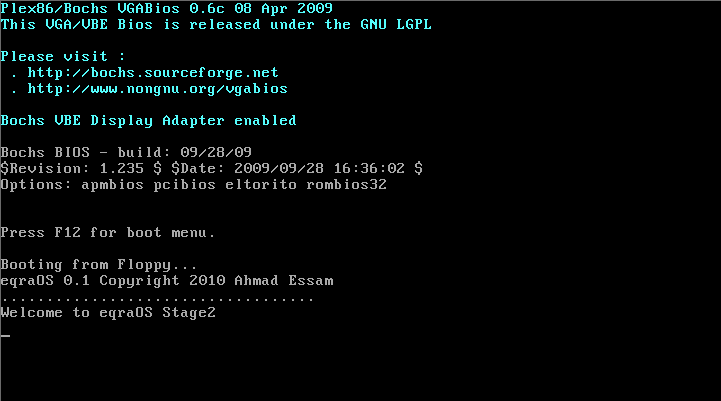
\includegraphics[width=0.9\textwidth]{../img/stage2}
\end{figure}

\begin{figure}[h!]
  \caption{بدء تنفيذ النواة}
    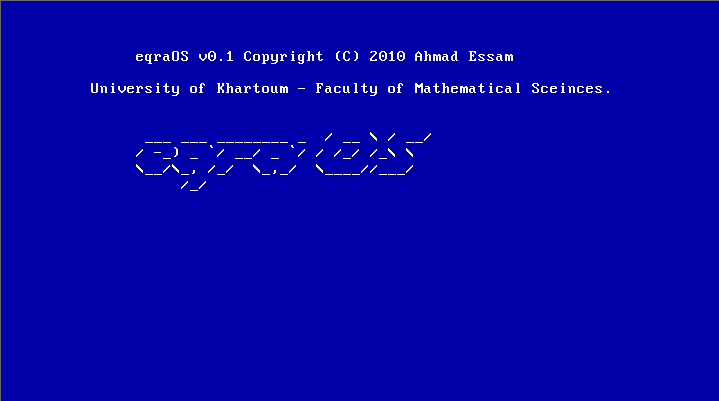
\includegraphics[width=0.9\textwidth]{../img/kernel}
\end{figure}


\end{document}
